\section{Dataset}

Multiple iterations of the recording process were run to find the best possible setup, which reduces the light interference as much as possible and which offers the best results with the resources at hand. The camera setup that is used by SilverFit was reproduced. At SilverFit the camera is mounted at $175cm$ above the floor. The camera that is used has an accelerometer which was used to adjust the camera angle relative to the ground. The camera is angled downward at a $70^\circ$ angle. 



% \subsection{Analysis}

% An important aspect of the dataset is the structure and distribution of data and their labels. In total, REPLACE_WE recorded all 13 exercises, mentioned in Section \ref{sec:exercises}, twice. Each recording session consists of exactly 300 frames.

% If a joint cannot be detected by Nuitrack it automatically gets zero coordinates, i.e. every value is zero. This makes it easy to automatically label these joints as faulty, in particular with the error label $1$ - Joint Missing. However, for the rest of the errors each frame has to be manually inspected and each joint considered. Since this requires a lot of work REPLACE_WE reduced the labeled frames to 10 percent of the original size. Therefore, each exercise contains 30 frames and in total $30 \cdot 13 \cdot 2 = 720$ frames are labeled.

% When multiple persons are detected one person might be incorrectly detected in the background. While analysing the data REPLACE_WE pick the person that is not labeled as faulty whenever possible. For training and testing this is chosen at random. If a person is labeled as faulty each joint is marked as in an unrealistic position.

% \subsubsection{Distribution of Errors}

% An important factor in how well a model can be trained on data is the balance of the dataset. In this case, the dataset is balanced by the error labels. In Figure \ref{fig:statistics_err_dist} REPLACE_WE can see the distribution of errors in the dataset as a whole. REPLACE_WE see that most of the joints are not faulty, i.e. are in the position they are supposed be within a margin of error.

% \begin{figure}
%   \centering
%   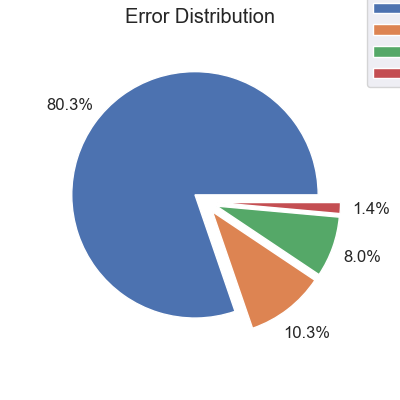
\includegraphics[width=0.5\textwidth]{figures/Data/Error_Distribution.png}
%   \caption[Error Distribution]{The distribution of errors TODO}
%   \label{fig:statistics_err_dist}
% \end{figure}

% To diversify the dataset REPLACE_WE recorded different exercises with varying difficulties. In Figure \ref{fig:statistics_err_diff} REPLACE_WE see that the difficulty has an influence on the amount of errors that occur for any given joint. REPLACE_WE see that there is barely any difference between the trivial and the easy exercises. However, in Figure \ref{fig:statistics_err_dist_diff} REPLACE_WE see that while trivial exercises have a higher percentage of unrealistic joint positions, i.e. the joint is in a wrong location, the easy exercises have a higher percentage of joints which are not detected. However, this difference is very small. Medium and Hard exercises are more error prone as was intended. This reflects REPLACE_OUR design proposals for challenging exercises from Section \ref{sec:exercises} indeed cause more difficult scenarios.

% \begin{figure}
%   \centering
%   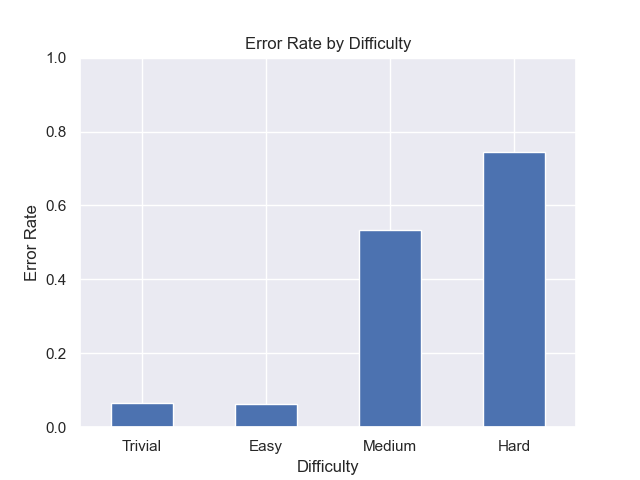
\includegraphics[width=0.5\textwidth]{figures/Data/Error_Rate_by_Difficulty.png}
%   \caption[Error Rate by Difficulty]{The rate that errors occur for any given difficulty. }
%   \label{fig:statistics_err_diff}
% \end{figure}

% \begin{figure}
%   \centering
%   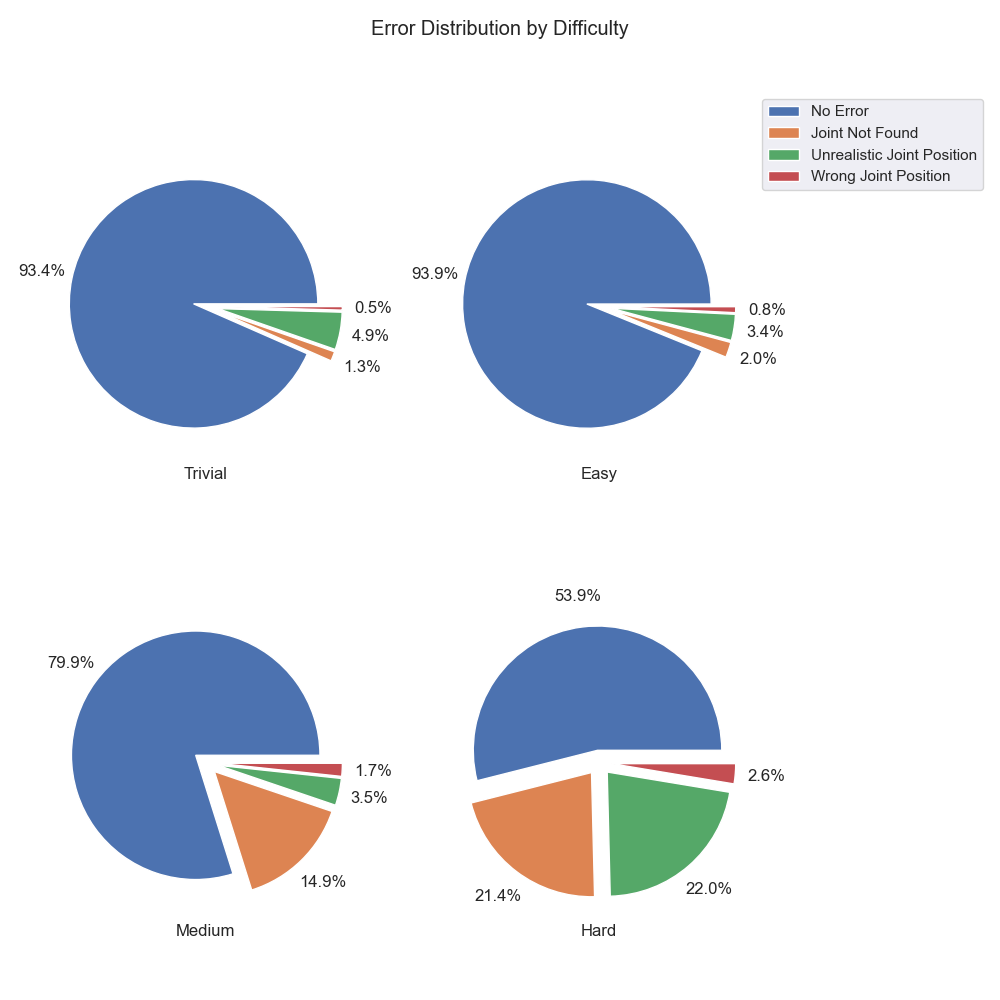
\includegraphics[width=0.5\textwidth]{figures/Data/Error_Distribution_by_Difficulty.png}
%   \caption[Error Distribution by Difficulty]{The distribution of errors by difficulty. TODO}
%   \label{fig:statistics_err_dist_diff}
% \end{figure}

% Some joints are more likely than others to be faulty, based on frequent occlusion, or generally more challenging detection. For example, hands and ankles are quite challenging to detect since they move frequently and are frequently occluded. On the other hand the head and the neck are least likely to be faulty. This distribution can be seen in Figure \ref{fig:statistics_err_dist_joint}, where the distribution of errors are shown for each joint. The joints are sorted by general occurrence of errors.

% \begin{figure}
%   \centering
%   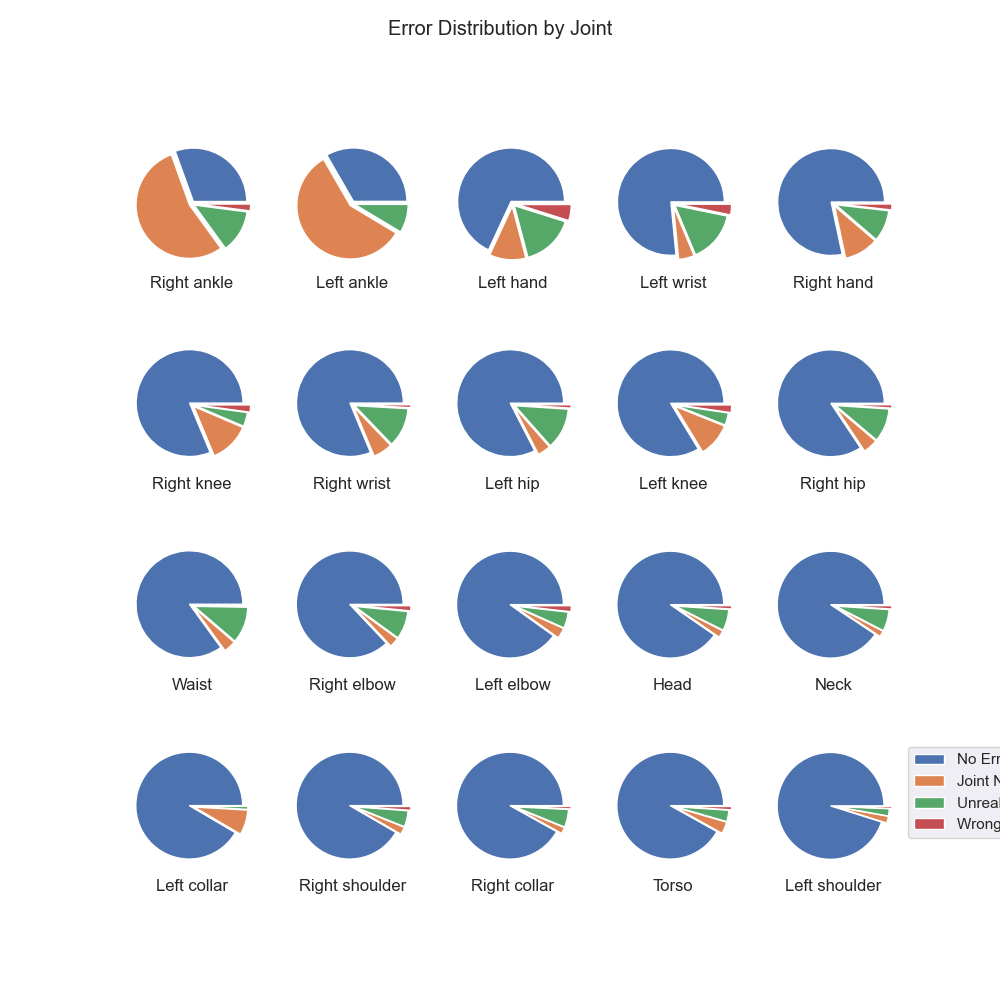
\includegraphics[width=0.5\textwidth]{figures/Data/Error_Distribution_by_Joint.png}
%   \caption[Error Distribution by Joint]{The distribution of errors by Joint. TODO}
%   \label{fig:statistics_err_dist_joint}
% \end{figure}

\subsection{Problem Sets}
\label{sec:problem_set}

Different problem sets are used to create different versions of the model. The problem sets are defined by the number of objects that are considered and are defined as erroneous. There are four different problem sets. The first problem set is the \textit{Joint} problem set. In this problem set, each joint is considered as a single object. The first simplification is to consider each joint, i.e. the individual arms, legs, torso, and head. The second simplification is to consider the upper and the lower body. Finally, only the whole body is considered.